\documentclass[10pt,twocolumn,letterpaper]{article}
\usepackage[pagenumbers]{cvpr}

\usepackage{graphicx}
\usepackage{amsmath,amssymb}
\usepackage{booktabs}
\usepackage[table]{xcolor}
\usepackage{tikz}
\usetikzlibrary{arrows.meta,calc}
\usepackage{cuted}
\usepackage{caption}
\captionsetup{font=small,skip=3pt}
\usepackage{microtype}
\usepackage{pifont}

\definecolor{cvprblue}{rgb}{0.21,0.49,0.74}
\usepackage[breaklinks,colorlinks,allcolors=cvprblue]{hyperref}

\def\paperID{FFI26}
\def\confName{CVPR}
\def\confYear{2026}

\title{Language-Gated GR-ConvNet: Steering a Lightweight Grasp Detector\\with CLIP Patch--Text Similarity}
\author{Minh-Ngoc Luong\\
Hanoi University of Science and Technology\\
{\tt\small ngoclm004@gmail.com}}

\begin{document}
\maketitle

\begin{strip}
\centering
\vspace{-2.0em}
\resizebox{\textwidth}{!}{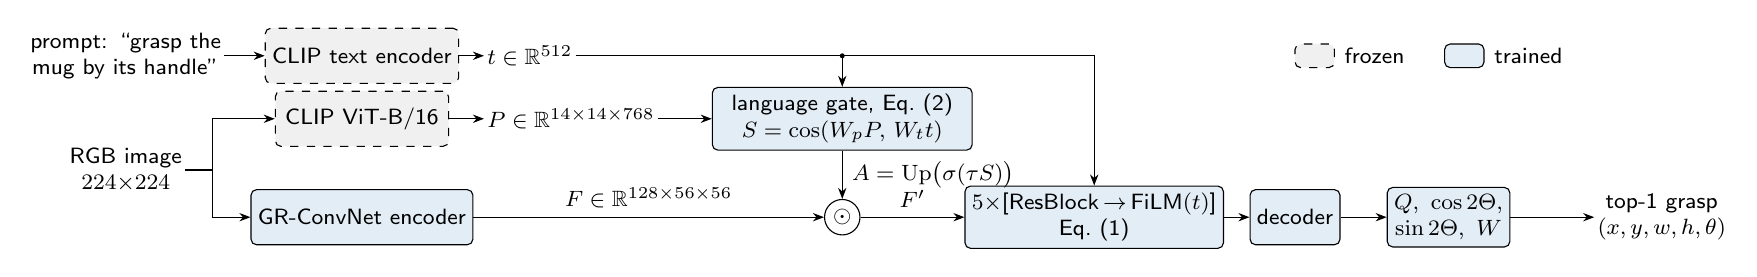
\begin{tikzpicture}[
  font=\sffamily\footnotesize, >={Stealth[length=4pt]},
  blk/.style={draw, rounded corners=2pt, align=center, minimum height=7mm, inner sep=2.5pt},
  frz/.style={blk, fill=gray!12, dashed},
  trn/.style={blk, fill=cvprblue!14},
  ten/.style={align=center, inner sep=1pt},
  op/.style={draw, circle, fill=white, inner sep=0pt, minimum size=4.5mm}]
  % ---- inputs
  \node[ten] (img) at (0.9,-0.0) {RGB image\\$224{\times}224$};
  \node[ten] (txt) at (0.9,1.45) {prompt: ``grasp the\\mug by its handle''};
  % ---- language lane (y=1.75)
  \node[frz, minimum width=22mm] (ctext) at (3.9,1.45) {CLIP text encoder};
  \node[ten, anchor=west] (t) at (5.45,1.45) {$t\in\mathbb{R}^{512}$};
  % ---- CLIP vision lane (y=0.65)
  \node[frz, minimum width=22mm] (cvis) at (3.9,0.65) {CLIP ViT-B/16};
  \node[ten, anchor=west] (P) at (5.45,0.65) {$P\in\mathbb{R}^{14\times14\times768}$};
  \node[trn, minimum width=33mm] (gate) at (10.0,0.65) {language gate, Eq.~(2)\\$S=\cos(W_pP,\,W_t t)$};
  % ---- geometry lane (y=-0.75)
  \node[trn, minimum width=22mm] (enc) at (3.9,-0.6) {GR-ConvNet encoder};
  \node[op] (mul) at (10.0,-0.6) {$\odot$};
  \node[trn, minimum width=30mm] (res) at (13.2,-0.6) {$5{\times}$[ResBlock$\,\rightarrow\,$FiLM$(t)$]\\Eq.~(1)};
  \node[trn] (dec) at (15.75,-0.6) {decoder};
  \node[trn] (heads) at (17.7,-0.6) {$Q,\ \cos2\Theta,$\\$\sin2\Theta,\ W$};
  \node[ten, anchor=west] (out) at (19.55,-0.6) {top-1 grasp\\$(x,y,w,h,\theta)$};
  % ---- arrows
  \draw[->] (txt) -- (ctext);
  \draw[->] (ctext) -- (t);
  \draw[->] (img.east) -- ++(0.35,0) |- (cvis.west);
  \draw[->] (img.east) -- ++(0.35,0) |- (enc.west);
  \draw[->] (cvis) -- (P);
  \draw[->] (P) -- (gate);
  \draw[->] (enc) -- node[above]{$F\in\mathbb{R}^{128\times56\times56}$} (mul);
  \draw[->] (gate) -- node[right]{$A=\mathrm{Up}\big(\sigma(\tau S)\big)$} (mul);
  \draw[->] (mul) -- node[above]{$F'$} (res);
  \draw[->] (res) -- (dec);
  \draw[->] (dec) -- (heads);
  \draw[->] (heads) -- (out);
  \draw[->] (t.east) -- (13.2,1.45) -- (res.north);
  \draw[->] (10.0,1.45) -- (gate.north);
  \fill (10.0,1.45) circle (0.9pt);
  % legend
  \node[frz, minimum height=3mm, minimum width=5mm] (lf) at (16.0,1.45) {};
  \node[anchor=west] at (lf.east) {frozen};
  \node[trn, minimum height=3mm, minimum width=5mm] (lt) at (17.9,1.45) {};
  \node[anchor=west] at (lt.east) {trained};
\end{tikzpicture}
}
\captionsetup{hypcap=false}
\captionof{figure}{\textbf{Language-Gated GR-ConvNet.} Only the blue blocks are trained (2.9M parameters); CLIP~\cite{radford2021clip} is frozen. The prompt enters twice: a spatial language gate $A$ on the encoder output, and FiLM~\cite{perez2018film} channel modulation after every residual block. Control C0 uses a learned vector $q$ instead of $W_t t$.}
\label{fig:arch}
\vspace{-0.5em}
\end{strip}

\begin{abstract}
Language-driven grasp detection requires placing a grasp on the object part named by a free-form prompt. We steer GR-ConvNet, a lightweight grasp network, with FiLM and a \emph{language gate}: a spatial map given by the cosine similarity between frozen CLIP patch tokens and the prompt embedding. Trained on 36k Grasp-Anything++ images, the model reaches 68.6\% seen and 57.8\% unseen success (two-seed mean) on the annotated official test split. A gate that cannot read the prompt loses 9.9 unseen points, so about half of the gain over FiLM comes from prompt-dependent gating rather than stronger visual features. Code: \url{https://github.com/Ngoc-LM/language-gated-grasp}.
\end{abstract}

\section{Introduction}
A parallel-jaw grasp is a rotated rectangle $g=(x,y,w,h,\theta)$: centre, opening, jaw size and angle~\cite{jiang2011rectangle}. Language-driven grasp detection conditions $g$ on a prompt such as ``grasp the knife by its handle'', so the model must first find \emph{which} part is meant. Grasp-Anything++~\cite{vuong2024lgd} provides 1M images, over 10M such prompts and a diffusion model, LGD; we instead steer a small single-pass grasp CNN. Our contributions are (i) a \emph{language gate} that re-weights GR-ConvNet~\cite{kumra2020grconvnet} features by CLIP~\cite{radford2021clip} patch--text similarity, adding 0.33M parameters (\cref{fig:arch}); (ii) a controlled ablation, with a text-free gate and a second seed, that separates the effect of CLIP visual features from that of prompt-dependent gating; and (iii) a leakage-controlled evaluation with open code.

\section{Related Work}
GG-CNN~\cite{morrison2018ggcnn} and GR-ConvNet~\cite{kumra2020grconvnet} regress dense grasp maps and decode the best pixel. CLIPort~\cite{shridhar2021cliport} fuses CLIP features into ``what/where'' streams for manipulation. Grasp-Anything++~\cite{vuong2024lgd} builds grasp data with foundation models, and LGD denoises grasps under text guidance. MaskCLIP~\cite{zhou2022maskclip} localises named objects with dense CLIP features; our gate instead learns lightweight projections that align CLIP patch tokens with the prompt.

\section{Method}
\textbf{Grasp maps.} As in~\cite{kumra2020grconvnet}, the network predicts four $224{\times}224$ maps: quality $Q$, $\cos2\Theta$, $\sin2\Theta$ and opening $W$. The angle is doubled because a grasp is unchanged by a $180^\circ$ rotation. Targets fill each ground-truth rectangle shortened to the central third of its opening. The smoothed maps are read at $\arg\max Q$, with $\theta=\tfrac12\operatorname{atan2}(\sin2\Theta,\cos2\Theta)$ and $h=w/2$.

\textbf{FiLM.} The encoder maps the image to $F\in\mathbb{R}^{128\times56\times56}$, followed by five residual blocks and a decoder. With $t$ the normalised CLIP text embedding, each residual block $k$ is followed by
\begin{equation}
F \leftarrow \big(1+\Delta\gamma_k(t)\big)\odot F + \beta_k(t),
\end{equation}
where $\Delta\gamma_k,\beta_k\in\mathbb{R}^{128}$ come from a zero-initialised linear layer, so each FiLM layer is the identity at initialisation.

\textbf{Language gate (proposed).} FiLM applies the same channel modulation at every pixel, so it can favour one object among several only indirectly. We therefore compare the $14{\times}14$ post-LayerNorm patch tokens $P$ of a frozen CLIP ViT-B/16 with the prompt and gate the encoder output:
\begin{equation}
\begin{gathered}
S_{ij}=\cos(W_p\,p_{ij},\,W_t\,t),\\
A=\mathrm{Up}_{56}\big(\sigma(\tau S)\big),\qquad F'=F\odot(1+A),
\end{gathered}
\end{equation}
with learned $W_p\in\mathbb{R}^{256\times768}$, $W_t\in\mathbb{R}^{256\times512}$ and temperature $\tau$ (initialised to 10). The residual form $1{+}A$ suppresses no feature but amplifies regions that match the prompt. The \textbf{C0 control} replaces $W_t t$ with a learned vector $q$: its gate sees the same CLIP features but not the prompt (FiLM still receives $t$). \textbf{Loss:} Smooth-$\ell_1$ summed over the four maps. Variant D adds $0.5\,\mathrm{BCE}(\tau S, M)$, where $M$ is the ground-truth $Q$ mask max-pooled to $14{\times}14$.

\section{Experiments}
\textbf{Protocol.} We train on 35,964 Grasp-Anything++ scenes (183,559 prompt--grasp pairs) and validate on 734. We test on the official LGD split (the 70\% most frequent LVIS categories are \emph{seen}), restricted to pairs with released annotations: 1,376 seen and 601 unseen pairs from 727 of its 803 object keys. All test scenes, and all training pairs whose object name is an unseen test object, are excluded from training. A top-1 grasp is correct if its IoU exceeds 0.25 and its angle error is below $30^\circ$ for some ground-truth grasp of the prompted part. $H$ is the harmonic mean of seen and unseen success. Decoding ground-truth maps scores 97.5\% (the encoding's ceiling). All models use AdamW (lr $10^{-3}$, weight decay $10^{-4}$, cosine), batch 32, 6 epochs, no augmentation and fp16 on one Kaggle T4 (2.5--2.7\,h); checkpoints are selected on 1,000 validation pairs.

\begin{figure}[t]
\centering
\setlength{\tabcolsep}{0.8pt}
\renewcommand{\arraystretch}{0.6}
\begin{tabular}{ccc}
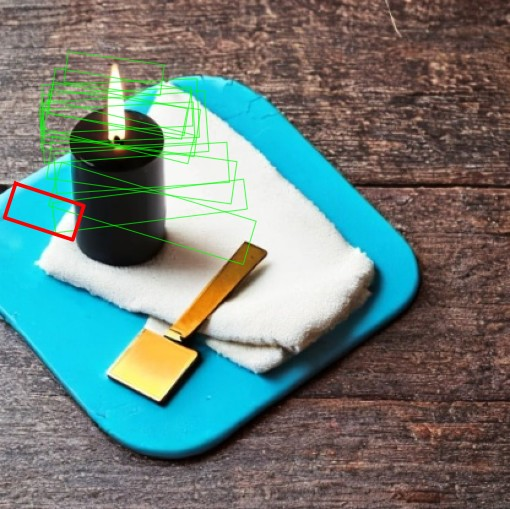
\includegraphics[width=0.3\linewidth]{fig/B_flame.jpg} &
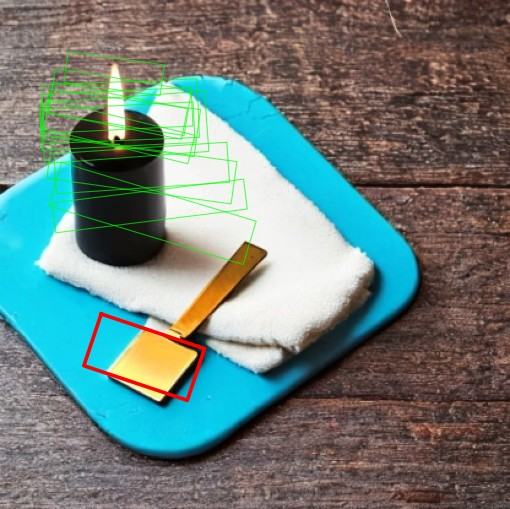
\includegraphics[width=0.3\linewidth]{fig/C0_flame.jpg} &
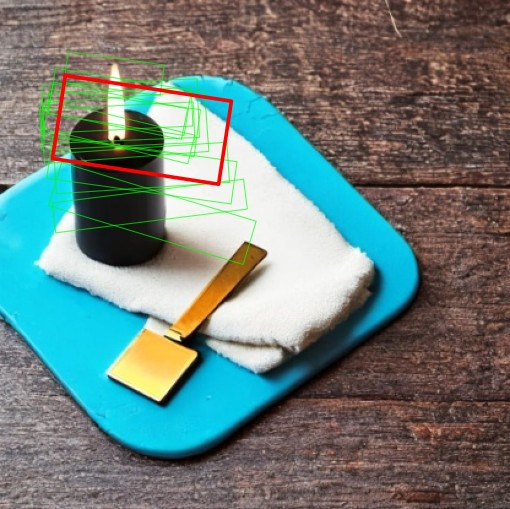
\includegraphics[width=0.3\linewidth]{fig/C_flame.jpg} \\
{\scriptsize B (FiLM) \ding{55}} & {\scriptsize C0 (text-free gate) \ding{55}} & {\scriptsize C (ours) \ding{51}}
\end{tabular}
\caption{\textbf{Selected unseen prompt} ``Fetch candle by its flame'' (green: GT, red: prediction). B misses the candle, C0 grasps a distractor, C grasps the named part. On ``lamp by its stand'', in contrast, C0 succeeds and C fails.}
\label{fig:qual}
\end{figure}

\begin{table}[t]
\centering
\small
\setlength{\tabcolsep}{2pt}
\begin{tabular}{@{}llcccc@{}}
\toprule
 & Model & Seen & Unseen & $H$ & ms \\
\midrule
A & GR-ConvNet (no text) & 27.3 & 27.8 & 27.5 & 4.3 \\
B & + FiLM$(t)$ & 52.0 & 40.1 & 45.3 & 12.3 \\
C0 & B + text-free CLIP gate & 62.8 & 47.9 & 54.4 & 18.2 \\
\rowcolor{cvprblue!10}
C & B + language gate (\textbf{ours}) & 68.6$_{\pm0.5}$ & 57.8$_{\pm1.9}$ & 62.8$_{\pm1.3}$ & 18.9 \\
D & C + gate supervision & 70.9 & 57.7 & 63.6 & 18.8 \\
\midrule
 & GR-ConvNet + CLIP$^\dagger$ & 37 & 18 & 24 & -- \\
 & LGD$^\dagger$~\cite{vuong2024lgd} & 48 & 42 & 45 & -- \\
\bottomrule
\end{tabular}
\caption{\textbf{Success rate (\%) on the test split.} C: mean${\pm}$half-range over two seeds; others: one seed. ms: end-to-end batch-1 latency on a T4, incl.\ CLIP. 95\% binomial intervals: ${\approx}\pm2.5$ (seen), $\pm3.9$ (unseen). $^\dagger$From~\cite{vuong2024lgd}, full training set; not directly comparable.}
\label{tab:main}
\end{table}

\textbf{Results.} \cref{tab:main} is a chain of controlled steps. Model A ignores the prompt and scores about equally on seen and unseen objects. FiLM (B) adds 17.8 points of $H$, and CLIP features behind a text-free gate (C0) add 9.1. Letting the gate read the prompt (C) adds 8.4 more, with a larger gain on unseen (+9.9) than seen (+5.9) objects, plausibly because CLIP's text embedding generalises to unseen names (\cref{fig:qual}). This unseen gap exceeds C's two-seed range (3.8) and the 95\% interval of a two-proportion difference ($\pm5.6$), so richer visual features alone do not explain it. Gate supervision (D) adds 2.2 seen points (within binomial noise) and leaves unseen and $H$ unchanged, so we keep the simpler C.

\textbf{Cost and limitations.} C also runs a frozen 149M-parameter CLIP; with the prompt embedding cached, a frame takes 12.5\,ms. We use 3.6\% of the images, one seed for most variants and only annotated test pairs, so absolute numbers are not directly comparable to~\cite{vuong2024lgd}.

\section{Conclusion}
A frozen-CLIP patch--text gate raises a lightweight grasp CNN from 27.5 to 62.8 $H$ under our protocol; about half of the gain over FiLM is due to making the gate prompt-dependent. Full-data training is the natural next step.

{\small
\bibliographystyle{ieeenat_fullname}
\bibliography{refs}
}

\end{document}
